\documentclass[11pt]{article}
\usepackage[T1]{fontenc}
\usepackage[margin=0.76in]{geometry}
\usepackage{amsmath,amssymb,amsthm}
\usepackage{graphicx}
\usepackage[hidelinks]{hyperref}
\usepackage{microtype}

\newtheorem{theorem}{Theorem}
\newcommand{\R}{\mathbb R}
\newcommand{\elltwo}{\ell^2}

\title{The positive difference space need not be closed:\\
a Hilbert lattice-cone counterexample}
\author{New counterexample for arXiv:1501.06696}
\date{13 August 2026}

\begin{document}
\maketitle

\paragraph{Status.}
\textbf{Full negative answer, in a strengthened form.}
There is a real Hilbert ordered gradient space for which
\(V_0=V_+-V_+\) is a proper dense subspace of \(V\), hence is not closed.
Moreover, both \(V_+\) and \(V_0\) are lattices, so the counterexample also
fits the lattice setting immediately surrounding the source question.

\section*{Source question}
Arnlind, Bj\"orn and Bj\"orn define
\[
 V_0=\{u\in V:u\le v\text{ for some }v\in V_+\}=V_+-V_+.
\]
After proving that this is a linear subspace, they state that they do not
know whether it is always closed [1, p.~19].

\begin{center}
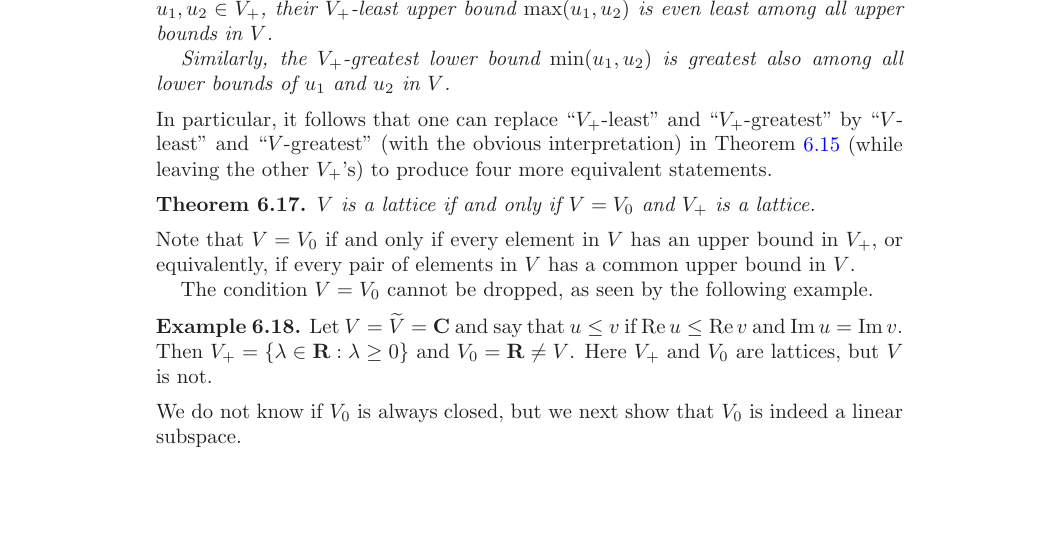
\includegraphics[width=0.95\textwidth]{figures/open_question_page19.png}
\end{center}
\noindent\emph{Source evidence: arXiv:1501.06696, p.~19.}

\section*{Proof intuition}
In the \(n\)-th copy of \(\R^2\), take the positive wedge generated by two
vectors that become almost parallel:
\[
 p_n=(1,0),\qquad q_n=(1,1/n).
\]
The blockwise direct sum of these wedges is a closed positive cone in a
Hilbert space.  Yet writing a vector as a difference of positive vectors
requires its coordinates in the increasingly ill-conditioned bases
\((p_n,q_n)\) to remain square summable.  This produces a dense graph-domain
inside the Hilbert space rather than a closed subspace.  The particularly
transparent witness has blocks \(q_n-p_n=(0,1/n)\): the vector is square
summable, but its coefficient sequences are the nonsummable constants
\((-1)\) and \(1\).

The wedges are acute, so adding a positive vector cannot decrease the
Hilbert norm.  Their basis coordinates also make maxima and minima
coordinatewise, which preserves the lattice property.

\begin{theorem}\label{thm:main}
There exists a real ordered gradient space
\(\mathcal U=(V,\widetilde V,W,\widetilde W,R)\) such that its positive
cone \(V_+\) is a lattice and
\[
 V_0=V_+-V_+
\]
is a proper dense, nonclosed vector subspace of \(V\).  The space \(V\) can
be chosen to be a Hilbert space, and \(V_0\) itself is a vector lattice.
\end{theorem}

\begin{proof}
Let
\[
 H=\elltwo(\mathbb N;\R^2)
\]
with its usual real Hilbert norm.  For \(n\ge1\), set
\[
 p_n=(1,0),\qquad q_n=(1,1/n),\qquad
 C_n=\{a p_n+bq_n:a,b\ge0\}\subset\R^2,
\]
and define
\[
 K=\{z=(z_n)\in H:z_n\in C_n\text{ for every }n\}.
\]
Each \(C_n\) is a closed, convex, pointed cone.  Since the coordinate
projections \(H\to\R^2\) are continuous, \(K\), their inverse-image
intersection, is also a closed, convex, pointed cone.  It defines a partial
order on \(H\) by \(u\le v\) exactly when \(v-u\in K\).

This order is compatible with the Hilbert norm.  Indeed, every two vectors
of \(C_n\) have nonnegative inner product: all four inner products among
the generators \(p_n,q_n\) are positive.  Hence
\(\langle u,w\rangle_H\ge0\) for \(u,w\in K\).  If \(0\le u\le v\), write
\(v=u+w\) with \(w\in K\); then
\[
 \|v\|_H^2=\|u\|_H^2+2\langle u,w\rangle_H+\|w\|_H^2
 \ge \|u\|_H^2.
\]

We now compute \(K-K\).  Every block has unique (real) coordinates
\begin{equation}\label{eq:coords}
 z_n=r_np_n+s_nq_n=(r_n+s_n,s_n/n),
 \qquad s_n=nz_{n,2},\quad r_n=z_{n,1}-nz_{n,2}.
\end{equation}
If \(k\in K\) has nonnegative coefficients \(a_n,b_n\), then
\(k_{n,1}=a_n+b_n\).  Thus \(k\in H\) implies
\((a_n),(b_n)\in\elltwo\).  It follows that if \(z=k-\ell\in K-K\), then
both coefficient sequences \((r_n),(s_n)\) in \eqref{eq:coords} belong to
\(\elltwo\).  Conversely, if \(r,s\in\elltwo\), splitting each into
positive and negative parts writes
\[
 z=(r^+p+s^+q)-(r^-p+s^-q)
\]
as the difference of two elements of \(K\).  Consequently,
\begin{equation}\label{eq:v0}
 K-K=\{z\in H:(r_n),(s_n)\in\elltwo\}
     =\{z\in H:(nz_{n,2})\in\elltwo\}.
\end{equation}
The last equality uses \((z_{n,1})\in\elltwo\).

The right-hand side of \eqref{eq:v0} contains every finitely supported
vector, so it is dense in \(H\).  It is not all of \(H\).  Namely, let
\[
 z^*_n=(0,1/n)=q_n-p_n.
\]
Then \(z^*\in H\), since \(\sum_n n^{-2}<\infty\), but its unique
coefficient sequences are \(r_n=-1\) and \(s_n=1\), which are not in
\(\elltwo\).  Thus \(z^*\notin K-K\).  Its finite truncations do belong to
\(K-K\) and converge to \(z^*\), explicitly witnessing nonclosedness.

For completeness, the construction preserves lattice structure.  In the
basis \((p_n,q_n)\), the order in every block is coordinatewise.  A positive
element of \(K\) has two nonnegative \(\elltwo\)-coefficient sequences, so
coordinatewise maxima and minima of two such elements again lie in \(K\).
Thus \(K\) is a lattice.  Formula \eqref{eq:v0} likewise shows that maxima
and minima of the coefficient pairs of two elements of \(K-K\) remain in
\(\elltwo\); hence \(K-K\) is a vector lattice.

Finally, turn this ordered Hilbert space into an ordered gradient space in
the source's sense.  Take
\[
 V=\widetilde V=W=\widetilde W=H,
 \qquad R=\{(u,u):u\in H\}.
\]
The identity relation is a closed linear gradient relation; the Hilbert
spaces are reflexive and strictly convex.  The preorder is compatible with
norm limits because \(K\) is closed, and the required norm monotonicity was
proved above.  Therefore this is an ordered gradient space.  Its positive
cone is \(V_+=K\), and its source-defined subspace is
\(V_0=V_+-V_+=K-K\), which is dense and nonclosed by the preceding
calculation.
\end{proof}

\small
\section*{Verification and literature status}
The bundled exact-arithmetic script checks the block-coordinate inverses,
acuteness on an exhaustive finite grid, the identity
\(q_n-p_n=(0,1/n)\), its coefficient pair \((-1,1)\), and convergence of
finite truncations.  These are independent sanity checks; the proof above
is complete without computation.

Exact-phrase, title, author, and ordered-gradient-space searches through
13 August 2026 found no later arXiv source answering this question.  This
was a bounded search rather than a systematic bibliographic review.

\subsection*{Reference}
\noindent [1] J. Arnlind, A. Bj\"orn and J. Bj\"orn,
\emph{An axiomatic approach to gradients with applications to Dirichlet and
obstacle problems beyond function spaces},
Commun. Contemp. Math. \textbf{18} (2016), 1550060;
arXiv:1501.06696.

\end{document}
